% Source: graduate-coursework/Research/Intro_to_Agents/handouts/Part4_Planning_Workflow.tex

\documentclass[border=4pt]{standalone}
\usepackage{graphicx}
\usepackage{tikz}
\usepackage{xcolor}
\usetikzlibrary{shapes.geometric, arrows.meta, positioning, calc, fit, backgrounds}

\definecolor{UofSCGarnet}{HTML}{73000A}
\definecolor{UofSCBlack}{HTML}{000000}
\definecolor{UofSCWhite}{HTML}{FFFFFF}
\definecolor{UofSCAtlantic}{HTML}{466A9F}
\definecolor{UofSCCongaree}{HTML}{1F414D}
\definecolor{UofSCHorseshoe}{HTML}{65780B}
\definecolor{UofSCRose}{HTML}{CC2E40}
\definecolor{UofSCDarkGarnet}{HTML}{570008}
\definecolor{UofSC90Black}{HTML}{363636}
\definecolor{UofSC70Black}{HTML}{5C5C5C}
\definecolor{UofSC50Black}{HTML}{A2A2A2}

\tikzset{
    box/.style={
        draw=UofSCBlack,
        fill=#1,
        minimum width=2.5cm,
        minimum height=0.8cm,
        text=UofSCWhite,
        font=\small\bfseries,
        align=center,
        inner sep=4pt
    },
    box/.default=UofSCGarnet,
    lightbox/.style={
        draw=UofSCBlack,
        fill=UofSCWhite,
        minimum width=2.5cm,
        minimum height=0.8cm,
        text=UofSCBlack,
        font=\small,
        align=center,
        inner sep=4pt
    },
    arrow/.style={
        ->,
        >=Stealth,
        thick,
        UofSCBlack
    },
    bigarrow/.style={
        ->,
        >=Stealth,
        line width=1.5pt,
        UofSCGarnet
    },
    phase/.style={
        draw=UofSCBlack,
        fill=#1,
        minimum width=3cm,
        minimum height=1cm,
        text=UofSCWhite,
        font=\bfseries,
        align=center
    },
    phase/.default=UofSCGarnet,
    subphase/.style={
        draw=UofSC70Black,
        fill=UofSCWhite,
        minimum width=2.8cm,
        minimum height=0.6cm,
        text=UofSCBlack,
        font=\scriptsize,
        align=center
    },
    cyclebox/.style={
        draw=UofSCBlack,
        line width=1.5pt,
        fill=#1,
        minimum width=2cm,
        minimum height=1.2cm,
        text=UofSCWhite,
        font=\bfseries,
        align=center
    },
    cyclebox/.default=UofSCGarnet
}

\begin{document}
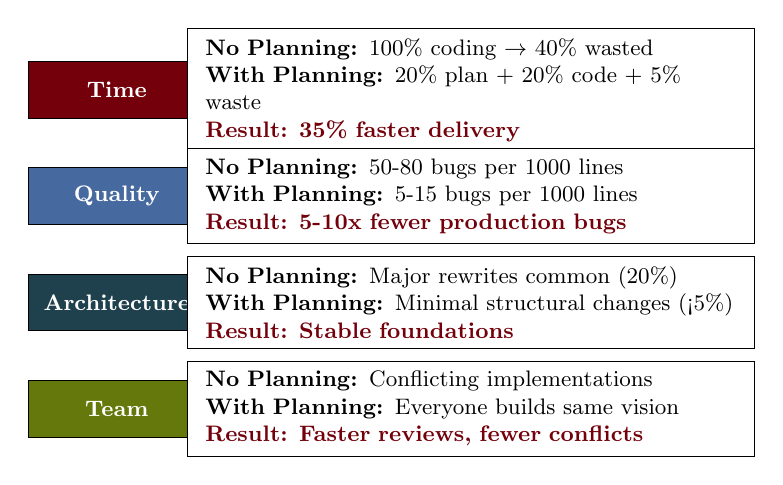
\begin{tikzpicture}[scale=0.9, transform shape]
        % Time efficiency
        \node[box=UofSCGarnet, minimum width=2.5cm] (t1) at (0,2.5) {Time};
        \node[lightbox, minimum width=8cm, text width=7.5cm, align=left] at (5,2.5) {
            \textbf{No Planning:} 100\% coding $\rightarrow$ 40\% wasted\\
            \textbf{With Planning:} 20\% plan + 20\% code + 5\% waste\\
            \textcolor{UofSCGarnet}{\textbf{Result: 35\% faster delivery}}
        };

        % Code quality
        \node[box=UofSCAtlantic, minimum width=2.5cm] (q1) at (0,1) {Quality};
        \node[lightbox, minimum width=8cm, text width=7.5cm, align=left] at (5,1) {
            \textbf{No Planning:} 50-80 bugs per 1000 lines\\
            \textbf{With Planning:} 5-15 bugs per 1000 lines\\
            \textcolor{UofSCGarnet}{\textbf{Result: 5-10x fewer production bugs}}
        };

        % Architecture
        \node[box=UofSCCongaree, minimum width=2.5cm] (a1) at (0,-0.5) {Architecture};
        \node[lightbox, minimum width=8cm, text width=7.5cm, align=left] at (5,-0.5) {
            \textbf{No Planning:} Major rewrites common (20\%)\\
            \textbf{With Planning:} Minimal structural changes (<5\%)\\
            \textcolor{UofSCGarnet}{\textbf{Result: Stable foundations}}
        };

        % Team
        \node[box=UofSCHorseshoe, minimum width=2.5cm] (team) at (0,-2) {Team};
        \node[lightbox, minimum width=8cm, text width=7.5cm, align=left] at (5,-2) {
            \textbf{No Planning:} Conflicting implementations\\
            \textbf{With Planning:} Everyone builds same vision\\
            \textcolor{UofSCGarnet}{\textbf{Result: Faster reviews, fewer conflicts}}
        };
    \end{tikzpicture}
\end{document}
